\begin{solution}
\begin{enumerate}
\item  A sample implementation of the hat function follows below.
       Student solutions should vary widely.
\small
\begin{verbatim}
 function phi_k = hat(x,k,N)

% function phi_k = hat(x,k,N)
%
% evaluates the hat function phi_k(x), where N denotes the
% size of the mesh, so that phi_k is non-zero on ((k-1)*h,(k+1)*h)
% with h = 1/(N+1). 

 h = 1/(N+1);
 xk = [0:N+1]*h;

 if k==0       
     phi_k =  ((x>=xk(1))&(x<xk(2))).*((xk(2)-x)/h);
 elseif k==N+1
     phi_k =  ((x>=xk(N+1))&(x<=xk(N+2))).*((x-xk(N+1))/h);
 else          
     phi_k =  ((x>=xk(k))&(x<xk(k+1))).*((x-xk(k))/h) ...
                       + ((x>=xk(k+1))&(x<xk(k+2))).*((xk(k+2)-x)/h);
 end
 \end{verbatim}
 \normalsize
 \item The MATLAB script to create the plot is given below.
       (It is acceptable for students to print their output in 
       black and white.)
 \small
\begin{verbatim}
%% Code for plotting hat functions
N=9;

k=[0 4 5 6 10]; % hat function indices
colors='bgrcmyk';
x=linspace(0,1,1000);
figure; hold on;
ct=0;  % initializing counter for loop
for j=k
    ct=ct+1;
    plot(x,hat(x,j,N),colors(ct));
    legendStr{ct}=['$\phi_{' num2str(j) '}(x)$'];
end
xlabel('$x$','interpreter','latex','fontsize',16);
ylabel('$\phi_k(x)$','interpreter','latex','fontsize',16);
title('Hat functions for various $k$','interpreter','latex','fontsize',16);
legend(legendStr,'interpreter','latex');
 \end{verbatim}
 \normalsize
\begin{figure}
\centering
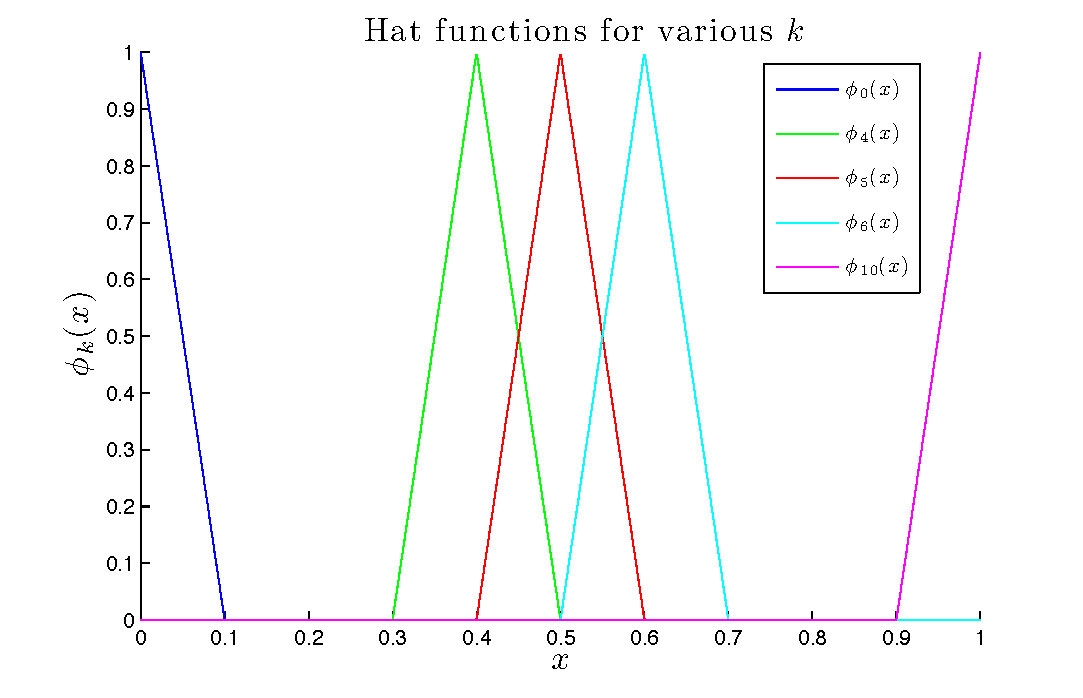
\includegraphics[width=.7\columnwidth]{./hatfxnsplot}
\caption{}
\end{figure}
 
\end{enumerate}
\end{solution}

